% Part: sets-functions-relations
% Chapter: arithmetization
% Section:reals

\documentclass[../../../include/open-logic-section]{subfiles}

\begin{document}

\olfileid[fa-IR]{sfr}{arith}{real}
\olsection{خط حقیقی}

گام بعدی آن است که نشان دهیم چگونه می‌توان اعداد حقیقی را از اعداد
گویا ساخت. پیش از آن، باید دریابیم چه چیزی در اعداد حقیقی
\emph{متمایز} است.

اعداد حقیقی بسیار شبیه اعداد گویا رفتار می‌کنند. (از نظر فنی، هر دو
نمونه‌هایی از \emph{میدان‌های مرتب} هستند؛ برای تعریف آن به
\olref[check]{orderedfield} بنگرید.) اکنون، اگر تمرین‌های
\olref[sfr][siz][]{chap} را انجام داده باشید، می‌دانید که شمار اعداد حقیقی
اکیداً بیش از شمار اعداد گویاست؛ یعنی $\cardless{\Rat}{\Real}$. کانتور
نخستین کسی بود که این مطلب را ثابت کرد. اما حدود دو هزاره و نیم است که
می‌دانیم اعداد گنگ وجود دارند؛ یعنی اعدادی حقیقی که گویا نیستند. در واقع:
%\footnote{Now: ``$\sqrt{2}$'' equally refers to both the positive and the negative roots; but in the next few pages, I'll forget about this, and consider only the positive root.}
\begin{thm}\ollabel{root2irrational}
$\sqrt{2}$ گویا نیست؛ یعنی $\sqrt{2} \notin \Rat$
\end{thm}

\begin{proof}
برای برهان خلف، فرض کنید $\sqrt{2}$ گویا باشد. پس $\sqrt{2} =
\nicefrac{m}{n}$ برای بعضی اعداد طبیعی $m$ و $n$. افزون بر این،
می‌توانیم $m$ و $n$ را چنان برگزینیم
که کسر بیش از این ساده‌کردنی نباشد. با بازآرایی، $m^{2} = 2n^{2}$.
از اینجا می‌توانیم برهان را به دو روش کامل کنیم:

\emph{نخست، به‌روش هندسی} (به پیروی از تننبام).\footnote{این
برهان را \cite{Conway2006} گزارش کرده است.} مربع‌های زیر را در نظر بگیرید:
\begin{center}
	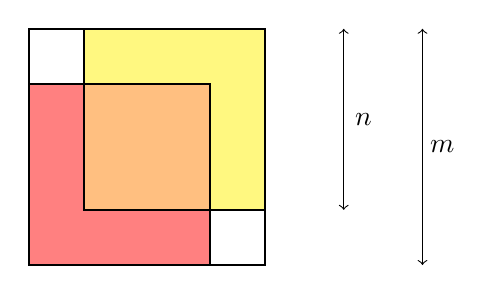
\begin{tikzpicture}
		\draw[thick] (0,0) rectangle (3,3);
		\draw[thick, fill=red!50] (0,0) rectangle (2.3,2.3);
		\draw[thick, fill=yellow!50] (0.7,0.7) rectangle (3, 3);
		\draw[thick, fill=orange!50] (0.7,0.7) rectangle (2.3, 2.3);
		\draw[<->] (4, 0.7)--(4, 3);
		\node at (4.25, 1.85) (n) {$n$};
		\draw[<->] (5, 0)--(5, 3);
		\node at (5.25, 1.5) (m) {$m$};
	\end{tikzpicture}
\end{center}
چون $m^2 = 2n^2$، ناحیهٔ هم‌پوشانیِ دو مربع با ضلع $n$ همان مساحتی
را دارد که ناحیهٔ بیرون از پوشش هر دو مربع؛ یعنی مساحت مربع نارنجی با
مجموع مساحت دو مربع بی‌رنگ برابر است. پس اگر مربع نارنجی ضلع $p$ و
هر مربع بی‌رنگ ضلع $q$ داشته باشد، $p^2 = 2q^2$. اما اکنون
$\sqrt{2} = \nicefrac{p}{q}$، که در آن $p < m$ و $q < n$ و $p, q \in
\Nat$. این نتیجه با این واقعیت تناقض دارد که $m$ و $n$ تا حد امکان
کوچک انتخاب شده بودند.

\emph{دوم، به‌روش صوری.} چون $m^{2} = 2n^{2}$، نتیجه می‌شود که $m$
زوج است. (به‌آسانی می‌توان نشان داد که اگر $x$ فرد باشد، آنگاه $x^2$
فرد است.) پس $m = 2r$، برای بعضی $r \in \Nat$. با بازآرایی،
$2r^2 = n^2$،
		%				\begin{align*}
		%					(2q)^{2} &= 2n^{2}\\
		%					4q^{2} &= 2n^{2}\\
		%					2q^{2} &= n^{2}
		%				\end{align*}
پس $n$ نیز زوج است. بنابراین $m$ و $n$ هر دو زوج‌اند و ازاین‌رو کسر
$\nicefrac{m}{n}$ را \emph{می‌توان} بیش از این ساده کرد. تناقض!
\end{proof}

در ضمن، این برهان نموداری به ما اجازه می‌دهد بار دیگر به مطالب
\olref[his][set][mythology]{sec} بازگردیم. تننبام (۱۹۲۷--۲۰۰۶)
ریاضی‌دانی کاملاً مدرن بود؛ بااین‌حال، این برهان بی‌تردید زیبا،
کاملاً دقیق و متکی بر شهود هندسی است!

در هر حال، اعداد حقیقی از اعداد گویا «گسترده‌ترند». به یک معنا، در
اعداد گویا «شکاف‌هایی» وجود دارد که اعداد حقیقی آن‌ها را پر می‌کنند.
وایرشتراس دریافت که این توصیف به خاصیتی یگانه از اعداد حقیقی اشاره
می‌کند که آن‌ها را از اعداد گویا متمایز می‌سازد: خاصیت تمامیت:
\emph{هر مجموعهٔ ناتهی از اعداد حقیقی که کران بالا داشته باشد، دارای
کوچک‌ترین کران بالا است.}

به‌آسانی می‌توان دید که اعداد گویا خاصیت تمامیت را ندارند. برای نمونه،
مجموعهٔ اعداد گویای کوچک‌تر از $\sqrt{2}$ را در نظر بگیرید؛ یعنی:
\[
	\Setabs{p \in \Rat}{p^2 < 2 \text{ or }p < 0}
\]
این مجموعه در اعداد گویا کران بالا دارد؛ برای نمونه، همهٔ !!{element}s<
آن از $3$ کوچک‌ترند. اما کوچک‌ترین کران بالای آن چیست؟ می‌خواهیم بگوییم
«$\sqrt{2}$»؛ ولی همین اکنون دیدیم که $\sqrt{2}$ \emph{گویا نیست}.
همچنین هیچ \emph{کوچک‌ترین} عدد گویای بزرگ‌تر از $\sqrt{2}$ وجود ندارد.
پس این مجموعه کران بالا دارد، اما کوچک‌ترین کران بالا ندارد. ازاین‌رو
اعداد گویا فاقد خاصیت تمامیت‌اند.

در مقابل، پیوستار «به‌لحاظ شهودی باید» خاصیت تمامیت داشته باشد. تنها
این را نمی‌خواهیم که $\sqrt{2}$ عددی حقیقی باشد؛ می‌خواهیم همهٔ
«شکاف‌های» خط گویا را پر کنیم. در واقع، می‌خواهیم خود پیوستار هیچ
«شکافی» نداشته باشد. تمامیت دقیقاً همین را برای ما فراهم خواهد کرد.

\end{document}
